
\subsection*{1.}

\begin{center}
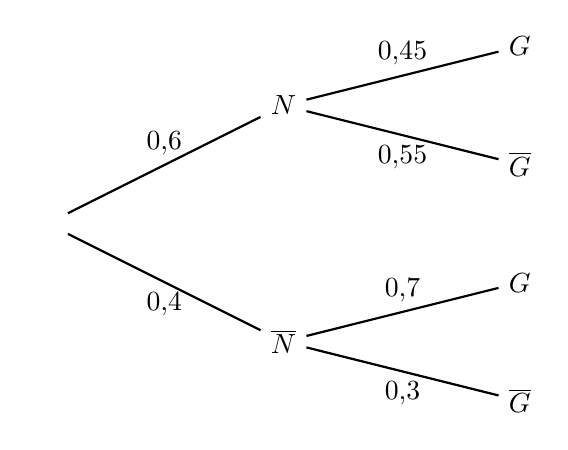
\begin{tikzpicture}[thick, scale=1.5] %{,}
\node (P_-1_0) at (-2,-1.5) {$\phantom{A}$};
\node (P_0_0) at (0,-0.5) {$N$};
\draw (P_-1_0) -- (P_0_0) node[midway, above] {$0{,}6$};
\node (P_1_0) at (2,-0) {$G$};
\draw (P_0_0) -- (P_1_0) node[midway, above] {$0{,}45$};
\node (P_1_1) at (2,-1) {$\overline{G}$};
\draw (P_0_0) -- (P_1_1) node[midway, below] {$0{,}55$};
\node (P_0_2) at (0,-2.5) {$\overline{N}$};
\draw (P_-1_0) -- (P_0_2) node[midway, below] {$0{,}4$};
\node (P_1_2) at (2,-2) {$G$};
\draw (P_0_2) -- (P_1_2) node[midway, above] {$0{,}7$};
\node (P_1_3) at (2,-3) {$\overline{G}$};
\draw (P_0_2) -- (P_1_3) node[midway, below] {$0{,}3$};
\end{tikzpicture}
\end{center}

\subsection*{2.}

On a :
\[
p(N \cap G) = p(N) \times p_N(G) = 0{,}6 \times 0{,}45 = 0{,}27.
\]

\subsection*{3.}

On a de même :
\[
p(\overline{N} \cap G) = p(\overline{N}) \times p_{\overline{N}}(G) = 0{,}4 \times 0{,}7 = 0{,}28.
\]
D'après la loi des probabilités totales :
\[
p(G) = p(N \cap G) + p(\overline{N} \cap G) = 0{,}27 + 0{,}28 = 0{,}55.
\]

\subsection*{4.}

Il faut trouver :
\begin{align*}
p_{\overline{G}}(N) &= \dfrac{p(\overline{G} \cap N)}{p(\overline{G})} \\
&= \dfrac{p(N \cap \overline{G})}{1 - p(G)} \\
&= \dfrac{0{,}6 \times 0{,}55}{1 - 0{,}55} \\
&= \dfrac{0{,}33}{0{,}45} \approx 0{,}733.
\end{align*}

\subsection*{5.}

On peut dresser un arbre représentant les résultats des deux combats :

\begin{center}
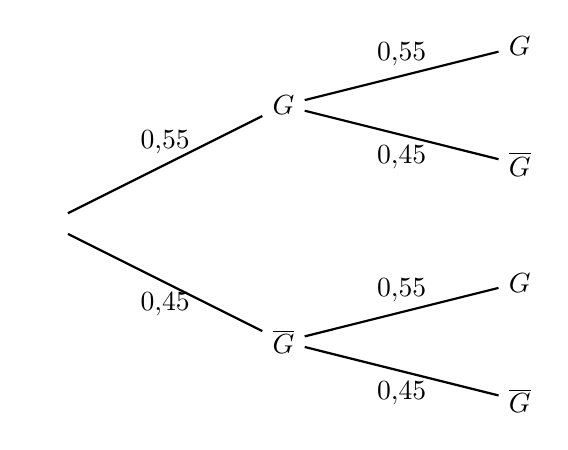
\begin{tikzpicture}[thick, scale=1.5] %{,}
\node (P_-1_0) at (-2,-1.5) {$\phantom{A}$};
\node (P_0_0) at (0,-0.5) {$G$};
\draw (P_-1_0) -- (P_0_0) node[midway, above] {$0{,}55$};
\node (P_1_0) at (2,-0) {$G$};
\draw (P_0_0) -- (P_1_0) node[midway, above] {$0{,}55$};
\node (P_1_1) at (2,-1) {$\overline{G}$};
\draw (P_0_0) -- (P_1_1) node[midway, below] {$0{,}45$};
\node (P_0_2) at (0,-2.5) {$\overline{G}$};
\draw (P_-1_0) -- (P_0_2) node[midway, below] {$0{,}45$};
\node (P_1_2) at (2,-2) {$G$};
\draw (P_0_2) -- (P_1_2) node[midway, above] {$0{,}55$};
\node (P_1_3) at (2,-3) {$\overline{G}$};
\draw (P_0_2) -- (P_1_3) node[midway, below] {$0{,}45$};
\end{tikzpicture}
\end{center}

On a :

\( p(G \cap G) = 0{,}55 \times 0{,}55 = 0{,}3025 \) ;

\( p\left(\overline{G} \cap \overline{G}\right) = 0{,}45 \times 0{,}45 = 0{,}2025 \).

Il reste donc pour la probabilité d'une victoire et une défaite (ou inversement) : 
\[
1 - (0{,}3025 + 0{,}2025) = 1 - 0{,}505 = 0{,}495.
\]
D'où le tableau de la loi de probabilité de \( X \) :

\[
\begin{array}{|c|c|c|c|}
\hline
\text{Valeur de } X : x_i & 0 & 1 & 2 \\
\hline
p(X = x_i) & 0{,}2025 & 0{,}495 & 0{,}3025 \\
\hline
\end{array}
\]

